\chapter{矩阵在平面几何中的应用}
\begin{proverb}
  { \itshape
   Everyone wants to teach and nobody wants to learn.
  }

\hfill Niels Abel(1802--1829)
\end{proverb}


\section{线性变换}
\begin{definition}
  设$A\in\MM_2(\MR)$. 函数$f_A:\MR^2\to\MR^2$定义为
  \[
    f_A(x,y) = (x',y'),\quad \text{其中}\quad
    \begin{pmatrix}
      x' \\ y'
    \end{pmatrix} = A \begin{pmatrix}
      x \\ y
    \end{pmatrix},
  \]
  称为是一个$\MR^2$上的由矩阵$A$定义的{\kaishu 线性变换}\index{X!线性变换}(或者由$A$定义的{\kaishu 线性映射}\index{X!线性映射}).

  矩阵$A$称为线性变换$f_A$的在标准基下的矩阵,记为$A_f$.
\end{definition}

\begin{prop}
  线性变换$f_A:\MR^2\to\MR^2,f_A(x,y)=(x',y')$,其中
  \[
    \begin{pmatrix}
      x' \\ y'
    \end{pmatrix} = A \begin{pmatrix}
      x \\ y
    \end{pmatrix}, \quad A\in \MM_2(\MR),
  \]
  具有如下性质:
  \begin{enum}
    \item\label{prop5.1a} $f_A\big( (x_1,y_1) + (x_2,y_2) \big)
    =f_A(x_1,y_1)+f_A(x_2,y_2),\,\forall (x_1,y_1),(x_2,y_2)\in\MR^2$;
    \item\label{prop5.1b} $f\big(\alpha(x_1,y_1)\big)=\alpha f_A(x_1,y_1),\,\forall\alpha\in\MR,\forall (x_1,y_1)\in\MR^2$,
  \end{enum}
  其中,$\MR^2$在注 \ref{remark1.3} 中为单行矩阵或(单列矩阵)定义的运算下构成一个实向量空间.
\end{prop}

\begin{proof}
  \begin{inparaenum}[(a)]
    \item 我们有
    \[
      A \left[ \begin{pmatrix}
        x_1 \\
        y_1
      \end{pmatrix} + \begin{pmatrix}
        x_2 \\
        y_2
      \end{pmatrix} \right] = A\begin{pmatrix}
        x_1 + x_2 \\
        y_1 + y_2
      \end{pmatrix} = A\begin{pmatrix}
        x_1 \\
        y_1
      \end{pmatrix}
      + A\begin{pmatrix}
        x_2 \\
        y_2
      \end{pmatrix},
    \]
    于是 \ref{prop5.1a} 得证.

    \item 另一方面,
    \[
      A\alpha \begin{pmatrix}
        x \\
        y
      \end{pmatrix} = A\begin{pmatrix}
        \alpha x \\
        \alpha y
      \end{pmatrix} = \alpha A\begin{pmatrix}
        x \\
        y
      \end{pmatrix},
    \]
    命题得证.
  \end{inparaenum}
\end{proof}

\begin{remark}
  我们提及一下在命题 \ref{prop5.1} 中的性质  \ref{prop5.1a} 和 \ref{prop5.1b} 等价于
  \[
    f_A\big( \alpha(x_1,y_1) + \beta (x_2,y_2) \big) = \alpha f_A(x_1,y_1) + \beta f_A(x_2,y_2),
  \]
  对任意$\alpha,\beta\in\MR$和$\forall(x_1,y_1),(x_2,y_2)\in\MR^2$成立.
\end{remark}

我们还有以下性质:
\begin{itemize}
  \item 线性变换是保持零向量的:$f_A(0,0)=(0,0)$;
  \item $f_A\big(-(x,y)\big)=-f_A(x,y)$;
  \item 恒等映射:$f_{I_2}(x,y)=(x,y)$或$f_{I_2}=I_{\MR^2}$.
\end{itemize}

\begin{definition}
  {\kaishu 线性变换的核与像.} 集合
  \[
    \Ker f_A = \left\{ (x,y)\in\MR^2: f_A(x,y) = (0,0) \right\}
  \]
  称为$f_A$的{\kaishu 核}\index{X!线性变换!核},而集合
  \[
    \im f_A = \left\{ f_A(x,y):(x,y)\in\MR^2 \right\}
  \]
  称为$f_A$的{\kaishu 像}.\index{X!线性变换!像}
\end{definition}

因此,线性变换的核是$\MR^2$中由所有被$f_A$映为零($\MR^2$中的零向量)的点(向量)构成,而$f_A$的像是由$\MR^2$中所有被$f_A$在$\MR^2$中的点(向量)映射所得的点(向量)构成.

\begin{lemma}
  以下性质成立:
  \begin{enum}
    \item $f_A$的核是$\MR^2$的一个子空间.

    $\forall\alpha,\beta\in\MR$以及$\forall (x_1,y_1),(x_2,y_2)\in\Ker f_A$,我们有$\alpha(x_1,y_1)+\beta(x_2,y_2)\in\Ker f_A$;
    \item $f_A$的像是$\MR^2$的一个子空间.

    $\forall\alpha,\beta\in\MR$以及$\forall (x_1,y_1),(x_2,y_2)\in\im f_A$,我们有$\alpha(x_1,y_1)+\beta(x_2,y_2)\in\im f_A$.
  \end{enum}
\end{lemma}
\begin{proof}
  本引理的证明留给感兴趣的读者作为练习.
\end{proof}

\begin{theorem}
  如果$A,B\in\MM_2(\MR)$,而$f_A,f_B$是由$A,B$确定的线性变换,则函数$f_A\circ f_B:\MR^2\to\MR^2$是由$AB$确定的线性变换.
\end{theorem}
\begin{proof}
  如果$f_B(x,y)=(x',y')$且$f_A(x',y')=(x'',y'')$,则
  \[
    f_A\circ f_B(x,y) = f_A\big( f_B(x,y) \big) = f_A(x',y') = (x'',y''),
  \]
  其中
  \[
    \begin{pmatrix}
      x'' \\
      y''
    \end{pmatrix} = A
    \begin{pmatrix}
      x' \\
      y'
    \end{pmatrix}\quad \text{且}\quad
    \begin{pmatrix}
      x' \\
      y'
    \end{pmatrix} = B
    \begin{pmatrix}
      x \\
      y
    \end{pmatrix}.
  \]
  于是
  \[
    \begin{pmatrix}
      x'' \\
      y''
    \end{pmatrix} =
    AB\begin{pmatrix}
      x \\
      y
    \end{pmatrix},
  \]
  所以线性变换$f_A\circ f_B$的矩阵为$AB$.
\end{proof}

\section{特殊变换的矩阵}
在本节以及接下来的计算中,为了简化计算,我们将点$(x,y)\in\MR^2$写成向量$\begin{pmatrix}
  x \\ y
\end{pmatrix}$.

\begin{mybox}
  \begin{theorem}[线性变换的矩阵.]

    如果线性变换$f_A:\MR^2\to\MR^2,f_A\begin{pmatrix}
      x \\
      y
    \end{pmatrix}=A\begin{pmatrix}
      x \\
      y
    \end{pmatrix}$,其中$A\in\MM_2(\MR)$,满足
    \[
      f_A\begin{pmatrix}
        1 \\
        0
      \end{pmatrix} = \begin{pmatrix}
        a \\
        b
      \end{pmatrix}\quad \text{且} \quad
      f_A\begin{pmatrix}
        0 \\
        1
      \end{pmatrix} = \begin{pmatrix}
        c \\
        d
      \end{pmatrix},\quad \text{则} \; A = \begin{pmatrix}
        a & c \\
        b & d
      \end{pmatrix}.
    \]
  \end{theorem}
\end{mybox}

\begin{proof}
  设$A=\begin{pmatrix}
    m & n \\
    p & q
  \end{pmatrix}$,由于
  \begin{gather*}
    f_A\begin{pmatrix}
      1 \\
      0
    \end{pmatrix} =\begin{pmatrix}
    m & n \\
    p & q
  \end{pmatrix}\begin{pmatrix}
    1 \\
    0
  \end{pmatrix} =
  \begin{pmatrix}
    m \\
    p
  \end{pmatrix} =
  \begin{pmatrix}
    a \\
    b
  \end{pmatrix}, \\
  f_A\begin{pmatrix}
      0 \\
      1
    \end{pmatrix} =\begin{pmatrix}
    m & n \\
    p & q
  \end{pmatrix}\begin{pmatrix}
    0 \\
    1
  \end{pmatrix} =
  \begin{pmatrix}
    n \\
    q
  \end{pmatrix} =
  \begin{pmatrix}
    c \\
    d
  \end{pmatrix},
  \end{gather*}
  我们得到$A=\begin{pmatrix}
    a & c \\
    b & d
  \end{pmatrix}$,定理得证.
\end{proof}

利用定理 \ref{thm5.2},我们可以求出不同线性变换的矩阵.

{\noindent\kaishu 通过原点反射的矩阵.}

我们希望求出通过原点反射的矩阵. 这是一个线性变换,将点$M(x,y)$映为$M'(-x,-y)$,即$M$关于原点的对称点.

设$f_A:\MR^2\to\MR^2,f_A\begin{pmatrix}
  x \\
  y
\end{pmatrix}=A\begin{pmatrix}
  x \\
  y
\end{pmatrix}$,其中$A=\begin{pmatrix}
  a & c \\
  b & d
\end{pmatrix}$.

由于
\[
  f_A\begin{pmatrix}
    1 \\
    0
  \end{pmatrix} =
  \begin{pmatrix}
    -1 \\
    0
  \end{pmatrix}\quad \text{且} \quad
  f_A\begin{pmatrix}
    0 \\
    1
  \end{pmatrix} =
  \begin{pmatrix}
    0 \\
    -1
  \end{pmatrix},
\]
由定理 \ref{thm5.2},我们有$A=\begin{pmatrix}
  -1 & 0 \\
  0 & -1
\end{pmatrix}$就是通过原点反射的矩阵.

{\noindent \kaishu 通过$x$轴反射的矩阵}

现在我们求出通过$x$轴反射的矩阵. 这是一个线性变换,将点$M(x,y)$映为$M'(x,-y)$,即$M$关于$x$轴的对称点.

由于
\[
  f_A\begin{pmatrix}
    1 \\
    0
  \end{pmatrix} =
  \begin{pmatrix}
    1 \\
    0
  \end{pmatrix}\quad \text{且} \quad
  f_A\begin{pmatrix}
    0 \\
    1
  \end{pmatrix} =
  \begin{pmatrix}
    0 \\
    -1
  \end{pmatrix},
\]
由定理 \ref{thm5.2},我们有$A=\begin{pmatrix}
  1 & 0 \\
  0 & -1
\end{pmatrix}$就是通过$x$轴反射的矩阵.

{\noindent \kaishu 通过$y$轴反射的矩阵}

和前面的计算一样,我们可得通过$y$轴反射的矩阵为$A=\begin{pmatrix}
  -1 & 0 \\
  0 & 1
\end{pmatrix}$.

{\kaishu 绕原点旋转角度$\alpha$的旋转矩阵.}

设$\alpha\in(0,2\pi)$. 绕原点旋转角度$\alpha$的变换保持原点$O$不变(它将$O$映为$O$),且将点$M$映为点$M'$,使得线段$[OM]$和$[OM']$具有相同的长度,即$OM=OM'$且$\angle MOM'=\angle\alpha$,且这两个角度的朝向相同(如果$\alpha>0$,则旋转是逆时针;如果$\alpha<0$,则旋转是顺时针).

设$f_A:\MR^2\to\MR^2,f_A\begin{pmatrix}
  x \\ y
\end{pmatrix}=A\begin{pmatrix}
  x \\ y
\end{pmatrix}$,其中$A=\begin{pmatrix}
  a & c \\
  b & d
\end{pmatrix}$且$\alpha\ge0$.

我们有$x'=\cos(\theta+\alpha)=
\cos\theta\cos\alpha-\sin\theta\sin\alpha,\cos\theta=x,
\sin\theta=y$. 于是$x'=x\cos\alpha-y\sin\alpha$. 类似地,$y'=\sin(\theta+\alpha)=\sin\theta\cos\alpha
+\cos\theta\sin\alpha $,于是$y'=x\sin\alpha+y\cos\alpha$.

由于
\[
  f_A\begin{pmatrix}
    1 \\
    0
  \end{pmatrix} = \begin{pmatrix}
    \cos\alpha \\
    \sin\alpha
  \end{pmatrix} \quad \text{且}\quad
  f_A\begin{pmatrix}
    0 \\
    1
  \end{pmatrix} = \begin{pmatrix}
    -\sin\alpha \\
    \cos\alpha
  \end{pmatrix},
\]
由定理 \ref{thm5.2},我们有$A=\begin{pmatrix}
  \cos\alpha & -\sin\alpha \\
  \sin\alpha & \cos\alpha
\end{pmatrix}$是{\kaishu 绕原点旋转角度$\alpha$的旋转矩阵.}

我们已经将这个矩阵(见问题 \ref{problem1.61})记为 $R_\alpha=\begin{pmatrix}
  \cos\alpha & -\sin\alpha \\
  \sin\alpha & \cos\alpha
\end{pmatrix}$.

任意角度为$\alpha$的旋转是一个双射,且其逆是角度为$-\alpha$的旋转.

所有绕原点的旋转构成的集合在(变换)的复合下构成一个Abel群,称为{\kaishu 旋转群.} \index{Q!群!旋转群}

\begin{mybox}
  绕任意点$(x_0,y_0)$的旋转满足方程
  \[
    \left\{
      \begin{aligned}
        & x' = x_0 + (x - x_0)\cos\alpha - (y - y_0)\sin \alpha \\
        & y' = y_0 + (x - x_0)\sin\alpha + (y - y_0)\cos\alpha
      \end{aligned}
    \right..
  \]
\end{mybox}

{\noindent \kaishu 因子为$k$的均匀缩放矩阵.}

设$k\in\MR^\ast$,因子为$k$的均匀缩放是一个线性变换(几何变换),它将点$M$映成点$M'$,且使得$\overrightarrow{OM'}=k\overrightarrow{OM}$,其中$O$是坐标原点. 我们立刻得到点$M(x,y)$的像就是$M'(kx,ky)$.

设$f_A:\MR^2\to\MR^2,f_A\begin{pmatrix}
  x \\
  y
\end{pmatrix}=A\begin{pmatrix}
  x \\
  y
\end{pmatrix}$,其中$A=\begin{pmatrix}
  a & c \\
  b & d
\end{pmatrix}$. 由于
\[
  f_A \begin{pmatrix}
    1 \\
    0
  \end{pmatrix} =
  \begin{pmatrix}
    k \\
    0
  \end{pmatrix} \quad \text{且} \quad
  f_A\begin{pmatrix}
    0 \\
    1
  \end{pmatrix} =
  \begin{pmatrix}
    0 \\
    k
  \end{pmatrix},
\]
由定理 \ref{thm5.2},我们有$A=\begin{pmatrix}
  k & 0 \\
  0 & k
\end{pmatrix}$就是因子为$k$的均匀缩放矩阵.

\begin{remark}
  当$k=-1$时,均匀缩放就变成了通过原点的反射.
\end{remark}

我们提及一下,在几何上,因子为$k>0$的均匀缩放也叫做以原点为中心,比率为$k$的位似. 我们将因子为$k$的均匀缩放记为$\theta_{0,k} $,且我们有$\theta_{0,k}(x,y)=(kx,ky)$.

以$(x_0,y_0)$为中心,比率为$k$的位似记为$\theta_{(x_0,y_0),k}$,其定义为
\[
  \theta_{(x_0,y_0),k} (x,y) = \big( x_0 + k(x - x_0), y_0 + k(y - y_0) \big).
\]

设$f_A:\MR^2\to\MR^2,f_A\begin{pmatrix}
  x \\ y
\end{pmatrix}=A\begin{pmatrix}
  x \\ y
\end{pmatrix}$,其中$A=\begin{pmatrix}
  a & b \\
  c & d
\end{pmatrix}$.

{\noindent \kaishu 从$\MR^2$中的向量到$x$轴的正交投影矩阵}

由于点$M(x,y)$到$x$轴的投影是点$M'(x,0)$,我们得到
\[
  f_A \begin{pmatrix}
    1 \\
    0
  \end{pmatrix} = \begin{pmatrix}
    1 \\
    0
  \end{pmatrix} \quad \text{且} \quad
  f_A \begin{pmatrix}
    0 \\
    1
  \end{pmatrix} = \begin{pmatrix}
    0 \\
    0
  \end{pmatrix},
\]
由定理 \ref{thm5.2},我们有$A=\begin{pmatrix}
  1 & 0 \\
  0 & 0
\end{pmatrix}$是 从$\MR^2$中的向量到$x$轴的正交投影矩阵. \index{J!矩阵!正交投影矩阵}

{\noindent\kaishu 从$\MR^2$中的向量到$y$轴的正交投影矩阵}

类似地,我们可以得到$A=\begin{pmatrix}
  0 & 0 \\
  0 & 1
\end{pmatrix}$是从$\MR^2$中的向量到$y$轴的正交投影矩阵.

\section{平面投影和反射}
\begin{definition}
  满足$P\circ P=P$的线性变换$P:\MR^2\to\MR^2$称为平面的{\kaishu 投影}.
\end{definition}

\begin{remark}
  一个投影是一个幂等的线性变换,即$\underbrace{P\circ P\circ\cdots\circ P}_{n\,\text{次}}=P,\forall n\ge2$.
\end{remark}

\begin{theorem}
  如果投影$P:\MR^2\to\MR^2$由矩阵$A$定义,则矩阵$A$是幂等的,即$A^2=A$.
\end{theorem}
\begin{proof}
  由定理 \ref{thm5.1},我们有$A_{P\circ P}=A_PA_P=A_P^2$,于是$A^2=A$.
\end{proof}

要求出平面上的所有投影,我们首先需要求出它们关联的矩阵,即幂等矩阵.
\begin{mybox}
  \begin{theorem}[实幂等矩阵.]

    矩阵$A=\begin{pmatrix}
      a & b \\
      c & d
    \end{pmatrix}\in\MM_2(\MR)$是幂等的当且仅当它具有以下形式之一:
    \begin{enum}
      \item $A_1=O_2$;
      \item $A_2=I_2$;
      \item $A_3=\begin{pmatrix}
        0 & 0 \\
        c & 1
      \end{pmatrix},x\in\MR$;
      \item $A_4=\begin{pmatrix}
        1 & 0 \\
        c & 0
      \end{pmatrix},c\in\MR$;
      \item $A_5=\begin{pmatrix}
        a & b \\
        \frac{a-a^2}b & 1 - a
      \end{pmatrix},a\in\MR,b\in\MR^\ast$.
    \end{enum}
  \end{theorem}
\end{mybox}
\begin{proof}
  见问题 \ref{problem1.14} 的解答.
\end{proof}

接下来的定理给出了平面上所有投影的几何解释.

\begin{mybox}
  \begin{theorem}[平面投影.]

    平面上的投影是线性映射$P_1,P_2,P_3,P_4,P_5:\MR^2\to\MR^2$,其定义为
    \begin{enum}\parindent=2em
      \item $P_1(x,y)=(0,0)$(零投影,平面上的所有点都投影到原点);
      \item $P_2(x,y)=(x,y)$(恒等变换);
      \item $P_3(x,y)=(0,cx+y)$(沿着直线$cx+y=0$的方向到$y$轴的斜投影);

          点$M(x,y)$被投影到$y$轴上, 连接点$(x,y)$和它的像$P(x,y)=(x',y')$的直线具有相同的斜率
          \[
            m = \frac{y'-y}{x'-x} = \frac{cx+y-y}{-x} = -c\quad \text{(常数)}.
          \]

          综上,$P_3$是沿着直线$cx+y=0$方向到$y$轴的斜投影.
      \item $P_4(x,y)=(x,cx)$(到直线$y=cx$的垂直投影);

          我们有$\im P_4=\{(x,cx):x\in\MR\}$,即此变换的像为直线$y=cx$. 由于点$(x,y)$和$(x,cx)$在同一条垂直的直线的上,我们得到$P_4$是到直线$y=cx$的垂直投影;

      \item $P_5(x,y)=\left(ax+by,\frac{a-a^2}bx+(1-a)y
          \right)$(沿着直线$cx+y=0$的方向到直线$y=\frac{1-a}bx$的斜投影);

          我们有
          \[
            \im P_5 = \left\{ \left( t,\frac{1-a}bt\right):t\in\MR \right\},
          \]
          于是此变换的像就是直线$y=\frac{1-a}bx$.

          连接点$M(x,y)$和它的像$P_5(x,y)=M'(x',y')$的直线斜率为
          \[
            m = \frac{y'-y}{x'-x} = - \frac ab \quad \text{(常数)}.
          \]
          综上,$P_5$是沿着直线$cx+y=0$的方向到直线$y=\frac{1-a}bx$的斜投影.
    \end{enum}
  \end{theorem}
\end{mybox}
\begin{proof}
  由定理 \ref{thm5.4} 即得.
\end{proof}

\begin{mybox}
  \begin{theorem}[投影的基本性质.]

    设$A\in\MM_2(\MR),A^2=A,A\ne O_2,A\ne I_2$,且令
    \[
      P_A : \MR^2 \to \MR^2,\quad P_A\begin{pmatrix}
        x \\
        y
      \end{pmatrix} =
      A\begin{pmatrix}
        x \\
        y
      \end{pmatrix}.
    \]
    则:
    \begin{enum}
      \item $\Ker P_A$是一条直线;
      \item $\im P_A$是一条直线;
      \item $P_A$沿着直线$\Ker P_A$的方向将点$(x,y)$投影到直线$\im P_A$上;
      \item 任意点$(x,y)\in\MR^2$可以唯一写成$\Ker P_A$中的一个点和$\im P_A$中的一个点的和(这意味着$\MR^2$是子空间$\Ker P_A$与$\im P_A$的直和,即$\MR^2=\Ker P_A\oplus \im P_A$);
      \item 幂等矩阵$A,A\ne O_2,A\ne I_2$的Jordan标准形为$J_A=\begin{pmatrix}
            1 & 0 \\
            0 & 0
          \end{pmatrix}$.
    \end{enum}
  \end{theorem}
\end{mybox}
\begin{proof}
  由定理的条件,我们可知$A$的秩为1,所以方程组$AX=0$有一个非平凡解$X_0\ne0$,此方程组的任意解形如$X=\alpha X_0,\alpha\in\MR$.
  \begin{enum}
    \item $\Ker P_A=\{(x,y);xy_0=yx_0\}$,其中$X_0=\begin{pmatrix}
          x_0 \\
          y_0
        \end{pmatrix}$.
    \item $Y\in\im P_A\Leftrightarrow$存在$X\in\MR^2$使得$AX=Y$,即非齐次方程组$AX=Y$是相容的. 这等价于$\rank(A|Y)=\rank (A)=1$,这意味着,如果$A_1$是$A$的一个非零列,则$Y=\alpha A_1,\alpha\in\MR$. 因此,对$A_1=\begin{pmatrix}
          a \\ c
        \end{pmatrix}$,我们有$\im P_A=\{(x,y):cx=ay\}$.
    \item 显然$P_A$将平面上的点映到直线$\im P_A$上,我们只需要证明连接平面上的一个点和它的像的向量平行于直线$\Ker P_A$,即向量$AX-X$与向量$X_0$成比例,其中$X_0$满足$AX_0=0$. 然而$A(AX-X)=A^2X-AX=(A^2-A)X=0$,这意味着向量$X_1=AX-X$是方程组$AX_1=0$的解,所以$X_1\in\Ker P_A$.
    \item 注意到任意点$(x,y)\in\MR^2$可以唯一写成$(x,y)=(x,y)-P_A(x,y)+P_A(x,y)$,其中$(x,y)-P_A(x,y)\in\Ker P_A$,而$P_A(x,y)\in\im P_A$.
  \end{enum}
  定理得证.
\end{proof}

\begin{definition}
  满足$S\circ S=I_{\MR^2}$(这意味着$S$是一个双射,且$S^{-1}=S$)的线性变换$S:\MR^2\to\MR^2$称为对合或者平面的{\kaishu 反射}.
\end{definition}

\begin{theorem}
  如果$S:\MR^2\to\MR^2$是一个由矩阵$A$定义的对合,则矩阵$A$是对合的,即$A^2=I_2$.
\end{theorem}
\begin{proof}
  由定理 \ref{thm5.1},我们有$A_{S\circ S}=A_SA_S=A_S^2$,于是$A^2=I_2$.
\end{proof}

要求出平面上的所有投影,我们首先需要求出它们关联的矩阵,即对合矩阵.

\begin{mybox}
  \begin{theorem}[实对合矩阵.]

    矩阵$B=\begin{pmatrix}
      a & b \\
      c & d
    \end{pmatrix}\in\MM_2(\MR)$是幂等的当且仅当它具有以下形式之一:
    \begin{enum}
      \item $B_1=-I_2$;
      \item $B_2=I_2$;
      \item $B_3=\begin{pmatrix}
        -1 & 0 \\
        c & 1
      \end{pmatrix},c\in\MR$;
      \item $B_4=\begin{pmatrix}
        1 & 0 \\
        c & -1
      \end{pmatrix},c\in\MR$;
      \item $B_5=\begin{pmatrix}
        a & b \\
        \frac{1-a^2}b & -a
      \end{pmatrix},a\in\MR,b\in\MR^\ast$.
    \end{enum}
  \end{theorem}
\end{mybox}
\begin{proof}
  见问题 \ref{problem1.12} 的解答.
\end{proof}

和投影的情形一样,下面的定理给出了平面上所有反射的几何解释.
\begin{mybox}
  \begin{theorem}[平面的反射.]

   平面上的投影是线性映射$S_1,S_2,S_3,S_4,S_5:\MR^2\to\MR^2$,其定义为
   \begin{enum}
     \item $S_1(x,y)=(-x,-y)$(通过原点的反射);
     \item $S_2(x,y)=(x,y)$(恒等变换);
     \item $S_3(x,y)=(-x,cx+y)$(直线$cx+2y=0$通过$y$轴方向的反射);
     \item $S_4(x,y)=(x,cx-y)$($y$轴通过直线$cx-2y=0$方向的反射);
     \item $S_5(x,y)=\left(ax+by,\frac{1-a^2}bx-ay\right)$
         (直线$(a+1)x+by=0$通过直线$(a-1)x+by=0$方向的反射).
   \end{enum}
  \end{theorem}
\end{mybox}
\begin{proof}
  由定理 \ref{thm5.8} 即得.
\end{proof}

\begin{mybox}
  \begin{theorem}[反射的基本性质.]

    设$A\in\MM_2(\MR),A^2=I_2,A\ne\pm I_2$,令
    \[
      S_A:\MR^2 \to \MR^2 ,\quad S_A\begin{pmatrix}
        x \\
        y
      \end{pmatrix} = A\begin{pmatrix}
        x \\
        y
      \end{pmatrix}.
    \]
    则:
    \begin{enum}
      \item 集合$\Inv S_A=\{(x,y)\in\MR^2:S_A(x,y)=(-x,-y)\}$是一条直线;
      \item 不动点集合$\Fix S_A=\{(x,y)\in\MR^2:S(x,y)=(x,y)\}$是一条直线;
      \item 对任意$X=\begin{pmatrix}
        x\\
        y
      \end{pmatrix}$,存在唯一的向量$X_1,X_2\in\MR^2$满足$AX_1=-X_1,AX_2=X_2$,且$X=X_1+X_2$;
      \item $S_A$是直线$\Inv S_A$方向通过直线$\Fix S_A$的反射;
      \item 任意点$(x,y)\in\MR^2$可以唯一写成$\Fix S_A$中的一个点和$\Inv S_A$中的一个点的和(这意味着$\MR^2$是子空间$\Fix S_A$与$\Inv S_A$的直和,即$\MR^2=\Fix S_A\oplus \Inv S_A$);
      \item 对合矩阵$A,A\ne\pm I_2$的的Jordan标准形为$J_A=\begin{pmatrix}
            1 & 0 \\
            0 & -1
          \end{pmatrix}$.
    \end{enum}
  \end{theorem}
\end{mybox}

\begin{proof}
  \begin{inparaenum}[(a)]
    \item 矩阵$A+I_2$的秩为1,所以方程组$AX=-X\Leftrightarrow(A+I_2)X=O_2$有非平凡解,所有非平凡解形如$\alpha X_0,X_0\in\MR^2,X_0\ne0$且$\alpha\in\MR$.

    \item 矩阵$A-I_2$的秩为1,所以方程组$AX=X\Leftrightarrow(A-I_2)X=O_2$有非平凡解,所有非平凡解形如$\beta X_1,X_1\in\MR^2,X_0\ne0$且$\beta\in\MR$.

    \item 如果存在这样的$X_1,X_2$,则$AX=AX_1+AX_2=-X_1+X_2$且$X=X_1+X_2$,所以$X_1=\frac12(X-AX)$且$X_2=\frac12(X+AX)$,这确实满足条件$AX_1=-X_1$和$AX_2=X_2$.

    \item 我们来证明连接一个点和它的像的直线的方向是固定的. 我们有$A(AX-X)=A^2X-AX=X-AX$,这意味着向量$X_1=AX-X$满足等式$AX_1=-X_1$,所以$X_1\in \Inv S_A$. 另一方面,$A\left(\frac12(AX+X)\right)=\frac12(A^2X+AX)
        =\frac12(X+AX)$,所以$X_2=\frac12(X+AX)$是一个不动点,即$AX_2=X_2$.

    \item 任意向量$v=(x,y)\in\MR^2$可以唯一写成$v=
    \frac12\big(v+S_A(v)\big)+\frac12\big(v-S_A(v)\big)$,其中$\frac12\big(v+S_A(v)\big)\in\Fix S_A$,且$
    \frac12\big(v-S_A(v)\big)\in\Inv S_A$.
  \end{inparaenum}
\end{proof}

现在,我们建立一个投影与对合之间的联系. 直觉上,我们有公式
\[
  P(x,y) = \frac12 \big( (x,y) + S(x,y) \big), \quad (x,y) \in \MR^2,
\]
这在几何上可以看成是点$P(x,y)$是由点$(x,y)$和$S(x,y)$确定的线段的中点.

\begin{mybox}
  \begin{theorem}[投影与对合之间的联系.]

    如果$P:\MR^2\to\MR^2$是一个投影,则$S=2P-I$是一个对合;反过来,如果$S:\MR^2\to\MR^2$是一个对合,则$P=\frac12(I+S)$是一个投影,其中$I:\MR^2\to\MR^2$是恒等映射.
  \end{theorem}
\end{mybox}

\begin{proof}
  设$P$的矩阵为$A\in\MM_2(\MR)$,$S$的矩阵为$B\in\MM_2(\MR)$,则$A^2=A$且$B^2=I_2$. 如果$B=2A-I_2$,则
  \[
    B^2 = 4A^2 - 4A + I_2 = 4A - 4A + I_2 = I_2.
  \]
  另一方面,如果$A=\frac12(I_2+B)$,则
  \[
    A^2 = \frac14(I_2 + 2B + B^2) = \frac14(I_2 + 2B + I_2) = \frac12(I_2 + B) = A,
  \]
  定理得证.
\end{proof}
\section{投影与反射的瑰宝}

在本节中,我们收集有关平面投影和反射的瑰宝和其他结果.

\begin{mybox}
  \begin{theorem}
    设$\mathscr D_1:ax+by=0$和$\mathscr D_2:cx+dy=0$是两条过原点的直线,其中$a^2+b^2\ne0,c^2+d^2\ne0,ad-bc\ne0$.
    \begin{enum}
      \item 沿着直线$\mathscr D_2$的方向到$\mathscr D_1$方向上的投影$P$是一个线性变换$P:\MR^2\to\MR^2$,其定义为
          \[
            P(x,y) = \left( \frac{-bcx - bdy}{ad - bc}, \frac{acx + ady}{ad - bc} \right).
          \]
      \item 直线$\mathscr D_2$通过直线$\mathscr D_1$方向的反射$S$是一个线性变换$S:\MR^2\to\MR^2$,其定义为
          \[
            S(x,y) = \left( \frac{-(ad+bc)x-2bdy}{ad-bc} ,
            \frac{2acx+(ad+bc)y}{ad-bc} \right).
          \]
    \end{enum}
  \end{theorem}
\end{mybox}
\begin{proof}
  对任意$(x,y)\in\MR^2$,存在唯一的$(x_1,y_1)\in\mathscr D_1$和$(x_2,y_2)\in\mathscr D_2$使得$(x,y)=(x_1,y_1)+(x_2+y_2)$. 由于$\im P=\Fix S=\mathscr D_1$,且$\Ker P=\Inv S=\mathscr D_2$,我们得到$P(x,y)=(x_1,y_1)$且$S(x,y)=(x_1,y_1)-(x_2,y_2)$.

  解方程组
  \[
    \left\{
      \begin{aligned}
        & ax_1 + by_1 = 0 \\
        & cx_2 + dy_2 = 0 \\
        & x_1 + x_2 = x \\
        & y_1 + y_2 = y
      \end{aligned}
    \right.,
  \]
  我们得到
  \[
    x_1 = \frac{-bcx-bdy}{ad-bc}, y_1 = \frac{acx+ady}{ad-bc}, x_2 = \frac{adx+bdy}{ad-bc}, y_2 = \frac{-acx-bcy}{ad-bc}.
  \]
  于是
  \[
    P(x,y) = \left( \frac{-bcx-bdy}{ad-bc},
    \frac{acx+ady}{ad-bc} \right),
  \]
  且
  \[
    S(x,y) = \left( \frac{-(ad+bc)x-2bdy}{ad-bc} ,
    \frac{2acx+(ad+bc)y}{ad-bc} \right).
  \]
  $P$和$S$的矩阵分别为
  \[
    M_P = \frac1{ad-bc} \begin{pmatrix}
      -bc & -bd \\
      ac & ad
    \end{pmatrix} \quad \text{和} \quad
    M_S = \frac1{ad-bc} \begin{pmatrix}
      -(ad + bc) & -2bd \\
      2ac & ad + bc
    \end{pmatrix}.
  \]
  定理得证.
\end{proof}

\begin{mybox}
  \begin{lemma}
    设$\mathscr D_1,\mathscr D_2,\mathscr D_3,\mathscr D_4$是四条过原点的直线,且满足$\mathscr D_1\perp \mathscr D_3,\mathscr D_2\perp\mathscr D_4$. 如果沿着直线$\mathscr D_2$的方向到直线$\mathscr D_1$的投影的矩阵是$M$,则沿着直线$\mathscr D_3$的方向到直线$\mathscr D_4$的投影的矩阵是$M\TT$.
  \end{lemma}
\end{mybox}
\begin{proof}
  设$\mathscr D_1:ax+by=0,\mathscr D_2:cx+dy=0,\mathscr D_3:-bx+ay=0,\mathscr D_4:-dx+cy=0$是引理中的四条直线. 由定理 \ref{thm5.12},我们有沿着直线$\mathscr D_2$的方向到直线$\mathscr D_1$的投影的矩阵为
  \[
    M = \frac1{ad-bc} \begin{pmatrix}
      -bc & -bd \\
      ac & ad
    \end{pmatrix},
  \]
  而沿着直线$\mathscr D_3$的方向到直线$\mathscr D_4$的投影的矩阵可以通过对矩阵$M$作变换$a\to-d,b\to c,c\to-b,d\to a$,我们得到
  \[
    \frac1{-ad+bc} \begin{pmatrix}
      bc & -ac \\
      bd & -ad
    \end{pmatrix} = \frac1{ad-bc} \begin{pmatrix}
      -bc & ac \\
      -bd & ad
    \end{pmatrix} = M\TT.
  \]
  
  类似地,我们可以证明,如果$A$是沿着直线$\mathscr D_2$的方向通过直线$\mathscr D_1$方向的反射的矩阵,则$A\TT$是沿着直线$\mathscr D_3$的方向通过直线$\mathscr D_4$方向的反射的矩阵.
\end{proof}

\begin{mybox}
  \begin{lemma}[线性映射何时为正交投影?]

    设$A\in\MM_2(\MR),A\ne O_2,A\ne I_2$,且设线性变换$f_A:\MR^2\to\MR^2$的矩阵为$A$. 则$f_A$是正交投影当且仅当$AA\TT=A$.
  \end{lemma}
\end{mybox}
\begin{proof}
  由于$AA\TT=A$,我们得到$AA\TT=A\TT$,这意味着$A=A\TT$. 因此,$A^2=A$,这说明$A$是一个幂等矩阵,且$f_A$是一个投影. 由引理 \ref{lemma5.2},如果$\mathscr D_1\perp \mathscr D_2$,则沿着直线$\mathscr D_2$的方向到直线$\mathscr D_1$的投影是正交的,所以$\mathscr D_3\equiv \mathscr D_2$,且$\mathscr D_4\equiv\mathscr D_1$. 于是$f_A$是正交投影当且仅当$A=A\TT$.
\end{proof}

\begin{mybox}
  \begin{nota}
    正交投影$P:\MR^2\to\MR^2$的矩阵为(见问题 \ref{problem5.8})
    \[
      M_P = \begin{pmatrix}
        a & b \\
        b & 1-a
      \end{pmatrix},\quad \text{$a,b\in\MR$满足$a^2+b^2=a$,}
    \]
    且$P(x,y)=\big(ax+by,bx+(1-a)y\big),\forall(x,y)\in\MR^2$.

    注意到这不是一个正交矩阵,即相应于正交投影的矩阵是{\kaishu 对称矩阵}而不是{\kaishu 正交矩阵}!
  \end{nota}
\end{mybox}

\begin{mybox}
  \begin{lemma}[投影及其矩阵.]

    设矩阵$A\in\MM_2(\MR)$的特征值为$\lambda_1=1$和$\lambda_2=0$,且相应的特征向量为$X_1=\begin{pmatrix}
      a \\
      b
    \end{pmatrix}$和$X_2=\begin{pmatrix}
      c \\
      d
    \end{pmatrix}$. 则$A$是沿着直线$\mathscr D_2:dx-cy=0$的方向到直线$\mathscr D_1:bx-ay=0$的投影的矩阵.
  \end{lemma}
\end{mybox}
\begin{proof}
  $A$的Jordan标准形为$J_A=\begin{pmatrix}
    1 & 0 \\
    0 & 0
  \end{pmatrix}$,相应的可逆矩阵$P=(X_1|X_2)=\begin{pmatrix}
    a & c \\
    b & d
  \end{pmatrix}$. 计算可得
  \[
    A = PJ_AP^{-1} = \frac1{ad-bc} \begin{pmatrix}
      ad & -ac \\
      bd & -bc
    \end{pmatrix}.
  \]
  通过在定理 \ref{thm5.12} 的证明最后的矩阵$M_P$的公式中替换$a\to b,b\to -a,c\to d,d\to -c$,我们得到此投影的矩阵$A$,引理得证.
\end{proof}

\begin{mybox}
  \begin{lemma}[反射及其矩阵.]

    设矩阵$B\in\MM_2(\MR)$的特征值为$\lambda_1=1$和$\lambda_2=-1$,相应的特征向量为$X_1=\begin{pmatrix}
      a \\
      b
    \end{pmatrix}$和$X_2=\begin{pmatrix}
      c \\
      d
    \end{pmatrix}$. 则$B$是沿着直线$\mathscr D_2:dx-cy=0$的方向通过直线$\mathscr D_1:bx-ay=0$的反射.
  \end{lemma}
\end{mybox}
\begin{proof}
  $B$的Jordan标准形为$J_B=\begin{pmatrix}
    1 & 0 \\
    0 & -1
  \end{pmatrix}$,相应的可逆矩阵$Q=(X_1|X_2)=\begin{pmatrix}
    a & c \\
    b & d
  \end{pmatrix}$,且$Q^{-1}=\dfrac1{ad-bc}\begin{pmatrix}
    d & -c \\
    -b & a
  \end{pmatrix}$.

  计算可得
  \[
    B = QJ_BQ^{-1} = \frac1{ad-bc} \begin{pmatrix}
      ad + bc & -2ac \\
      2bd & -(ad + bc)
    \end{pmatrix}.
  \]
  通过在定理 \ref{thm5.12} 的证明最后的矩阵$M_S$的公式中替换$a\to b,b\to -a,c\to d,d\to -c$,我们得到此反射的矩阵$B$,引理得证.
\end{proof}

\section{平面的等距}
\begin{definition}
  满足$T(x,y)=(x',y'),x^2+y^2=x'^2+y'^2$对任意$(x,y)\in\MR^2$的线性变换$T:\MR^2\to\MR^2$称为是平面的{\kaishu 线性等距}. \index{X!线性变换!线性等距}
\end{definition}

\begin{lemma}
  等距保持$\MR^2$中内积,保持点之间的距离和向量的夹角.
\end{lemma}

\begin{proof}
  如果$T(x_1,y_1)=(x_1',y_1')$且$T(x_2,y_2)=(x_1',y_2')$,我们需要证明
  \[
    x_1x_2 + y_1y_2 = x_1'x_2' + y_1'y_2'.
  \]

  我们有
  \[
    T(x_1+x_2,y_1+y_2) = (x_1'+x_2',y_1'+y_2'),
  \]
  且$(x_1+x_2)^2+(y_1+y_2)^2=(x_1'+x_2')^2+(y_1'+y_2')^2$.

  这意味着
  \[
    x_1^2 + 2x_1x_2 + x_2^2 + y_1^2 + 2y_1y_2 + y_2^2 = x_1'^2 + 2x_1'x_2' + x_2'^2 + y_1'^2 + 2y_1'y_2' + y_2'^2.
  \]
  由于$x_1^2+y_1^2=x_1'^2+y_1'^2$且
  $x_2^2+y_2^2=x_2'^2+y_2'^2$,我们得到$x_1x_2+y_1y_2=x_1'x_2'+y_1'y_2'$.

  如果$\alpha=\angle\big((x_1,y_1),(x_2,y_2)\big)$且
  $\alpha'=\angle \big( T(x_1,y_1),T(x_2,y_2) \big)$,则
  \[
    \cos\alpha = \frac{x_1x_2+y_1y_2}{\sqrt{x_1^2+y^2}
    \sqrt{x_2^2+y_2^2}} \quad \text{且} \quad
    \cos\alpha' = \frac{x_1'x_2'+y_1'y_2'}{\sqrt{x_1'^2+y_1'^2}
    \sqrt{x_2'^2+y_2'^2}},
  \]
  由定理的第一部分可知这两者是相等的.

  要证明$\dif\big((x_1,y_1),(x_2,y_2)\big)=
  \dif\big(T(x_1,y_1),T(x_2,y_2)\big)$,我们需要证明$(x_1-x_2)^2+(y_1-y_2)^2=(x_1'-x_2')^2+(y_1'-y_2')^2$,这等价于证明$x_1x_2+y_1y_2=x_1'x_2'+y_1'y_2'$.
\end{proof}

\begin{definition}
  如果函数$F:\MR^2\to\MR^2$保持点之间的距离,则它成为是一个等距,这里$F$不一定是线性变换.
\end{definition}

\begin{mybox}
  \begin{theorem}
    线性变换$T:\MR^2\to\MR^2$是一个等距当且仅当它的矩阵$M_T$具有以下形式之一:
    \[
      M_T = \begin{pmatrix}
        \cos t & -\sin t \\
        \sin t & \cos t
      \end{pmatrix} \quad \text{或} \quad
      M_T = \begin{pmatrix}
        \cos t & \sin t \\
        \sin t & -\cos t
      \end{pmatrix}.
    \]
  \end{theorem}
\end{mybox}
\begin{proof}
  设$M_T=\begin{pmatrix}
    a & b \\
    c & d
  \end{pmatrix}$. 我们有$T(x,y)=(x',y')=(ax+by,cx+dy)$,且
  \[
    x^2 + y^2 = (ax + by)^2 + (cx + dy)^2,\quad \forall (x,y) \in \MR^2.
  \]
  通过比较$x^2,y^2$和$xy$的系数,我们得到$a^2+c^2=1,b^2+d^2=1$,且$ab+cd=0$. 由于$a^2+c^2=1,b^2+d^2=1$,我们得到存在$t,s\in\MR$使得$\cos t=a,\sin t=c$以及$\cos s=d,\sin s=b$. 等式$ab+cd=0$意味着
  \[
    \cos t\sin s + \sin t \cos s = 0 \quad \Leftrightarrow \quad \sin(s + t) = 0,
  \]
  于是$t+s\in\{k\pi:k\in\MZ\}$.

  当$s+t=0$时,我们得到$s=-t$,这意味着$M_{T_1}=\begin{pmatrix}
    \cos t & -\sin t \\
    \sin t & \cos t
  \end{pmatrix}$.

  当$s+t=\pi$时,我们得到$s=\pi-t$,这意味着$M_{T_2}=\begin{pmatrix}
    \cos t & \sin t \\
    \sin t & -\cos t
  \end{pmatrix}$. 定理得证.
\end{proof}

\begin{remark}
  我们说明一下,矩阵
  \[
    M_ {T_1}=\begin{pmatrix}
      \cos t & -\sin t \\
      \sin t & \cos t
    \end{pmatrix}
  \]
  对应于一个角度为$t$的逆时针旋转,而矩阵
  \[
    M_ {T_2}=\begin{pmatrix}
      \cos t & \sin t \\
      \sin t & -\cos t
    \end{pmatrix}
  \]
  对应于一个旋转和一个反射的复合,即$M_{T_2}=M_{T_1}M_S$,其中$M_S=\begin{pmatrix}
    1 & 0 \\
    0 & -1
  \end{pmatrix}$表示关于$x$轴的反射.
\end{remark}

\begin{definition}
  设$(x_0,y_0)\in\MR^2$给定,函数$T_{(x_0,y_0)}:\MR^2\to\MR^2$定义为$T_{(x_0,y_0)}(x,y)=(x+x_0,y+y_0)$称为{\kaishu 向量$(x_0,y_0)$的平移}.
\end{definition}

因此,平移的公式为
\[
  T_{(x_0,y_0)}(x,y) = (x',y')\quad \Leftrightarrow \quad
  \left\{
     \begin{aligned}
       & x' = x_0 + x \\
       & y' = y_0 + y
     \end{aligned}
  \right..
\]
原点被平移到点$(x_0,y_0)$.

两个平移的复合是一个平移
\[
  T_{(x_0,y_0)}\circ T_{(x_0',y_0')} = T_{(x_0+x_0',y_0+y_0')},
\]
一个平移的逆也是一个平移$T^{-1}_{(x_0,y_0)}=T_{(-x_0,-y_0)}$.

我们指出,平移保持两点的距离和直线的夹角不变,将平行线变换到平行线,将圆变换成圆.

所有的平移的集合在复合运算下构成一个群,称为平面的{\kaishu 平移群}. \index{Q!群!平移群}

\begin{definition}
  如果$f:\MR^2\to\MR^2$是一个线性变换,而$T:\MR^2\to\MR^2$是一个平移,定义函数$g_1,g_2:\MR^2\to\MR^2$为$g_1=T\circ f$和$g_2=f\circ T$,称为{\kaishu 仿射变换}. \index{F!仿射变换}
\end{definition}

因此,仿射变换是由平移与线性变换复合而成.

如果$A=\begin{pmatrix}
  a & b \\
  c & d
\end{pmatrix}$是$f$的矩阵,而$(x_0,y_0)$是平移的向量,则$g(x,y)=(x',y')$,其中
\[
  \begin{pmatrix}
    x' \\
    y'
  \end{pmatrix} = A\begin{pmatrix}
    x \\
    y
  \end{pmatrix} +
  \begin{pmatrix}
    x_0 \\
    y_0
  \end{pmatrix},
\]
这意味着$g(x,y)=(ax+by+x_0,cx+dy+y_0),(x,y)\in\MR^2$,且
\begin{mybox}
  \[
    \left\{
      \begin{aligned}
        & x' = ax + by + x_0 \\
        & y' = cx + dy + y_0
      \end{aligned}
    \right.
  \]
  是仿射变换的公式.
\end{mybox}

所有仿射变换在函数的复合运算下构成一个群,称为{\kaishu 仿射变换群}. \index{Q!群!仿射变换群}

\section{平面的坐标方程组}
平面$\MR^2=\{(x,y):x,y\in\MR\}$上的标准{\kaishu 笛卡尔坐标系} $xOy$由两条垂直的直线构成,即$x$轴,$Ox=\{(x,0):x\in\MR\}$和$y$轴,
$Oy=\{(0,y):y\in\MR\}$,这两条线交于笛卡尔坐标系的原点$O(0,0)$.

将笛卡尔坐标系绕着原点逆时针旋转角度$\alpha$,我们得到一个新的坐标系,记为$x'Oy'$. 平面上的任一点$M$在坐标系$xOy$下被一组实数$(x,y)$唯一确定,同样的点在坐标系$x'Oy'$下被一组实数$(x',y')$所确定. 这两组实数互相关联的公式为
\[
  \begin{pmatrix}
    x \\
    y
  \end{pmatrix} =
  \begin{pmatrix}
    \cos\alpha & -\sin\alpha \\
    \sin\alpha & \cos\alpha
  \end{pmatrix}  \begin{pmatrix}
    x' \\
    y'
  \end{pmatrix}
\]
或者
\[
  \begin{pmatrix}
    x' \\
    y'
  \end{pmatrix} = \begin{pmatrix}
    \cos\alpha & \sin\alpha \\
    -\sin\alpha & \cos\alpha
  \end{pmatrix}
  \begin{pmatrix}
    x \\
    y
  \end{pmatrix},
\]
我们可以通过旋转矩阵$R_\alpha$或$R_{-\alpha}$从一个坐标系过渡到另一个坐标系.

通过平移坐标系$x'Oy'$,使得原点$O(0,0)$被平移到点$O''(x_0,y_0)$,我们得到平面上的一个新坐标系$x''O''y''$,则我们有公式
\[
  \begin{pmatrix}
    x'' \\
    y''
  \end{pmatrix} = R_{-\alpha} \begin{pmatrix}
    x - x_0 \\
    y - y_0
  \end{pmatrix}
\]
或
\[
  \begin{pmatrix}
    x \\
    y
  \end{pmatrix} =
  \begin{pmatrix}
    x_0 \\
    y_0
  \end{pmatrix} + R_\alpha
  \begin{pmatrix}
    x'' \\
    y''
  \end{pmatrix}.
\]

\begin{example}
  如果坐标系$x''O''y''$通过逆时针旋转笛卡尔坐标系$xOy$角度$\frac\pi6$得到,再将它平移到点$O''(1,2)$,则平面上在标准坐标系下坐标为$(x,y)$的点$M$在新坐标系$x''O''y''$下的坐标$(x'',y'')$之间满足
  \[
    \begin{pmatrix}
      x'' \\
      y''
    \end{pmatrix} = \begin{pmatrix}
      \frac{\sqrt3}2 & \frac12 \\
      -\frac12 & \frac{\sqrt3}2
    \end{pmatrix}
    \begin{pmatrix}
      x-1 \\
      y-2
    \end{pmatrix},
  \]
  或
  \[
    \begin{pmatrix}
      x \\
      y
    \end{pmatrix} =
    \begin{pmatrix}
      1 \\
      2
    \end{pmatrix} +
    \begin{pmatrix}
      \frac{\sqrt3}2 & -\frac12 \\
      \frac12 & \frac{\sqrt3}2
    \end{pmatrix}
    \begin{pmatrix}
      x'' \\
      y''
    \end{pmatrix}.
  \]
\end{example}

\section{问题}
\begin{problem}
  设$S_x$是通过$x$轴的反射,$S_y$是通过$y$轴的反射,求$S_x\circ S_y$的矩阵.
\end{problem}

\begin{problem}
  设$ABCDEF$是一个边长为2的正六边形,在直角坐标系$xCy$下,顶点$B$和$E$分别在$Cx$和$Cy$上. 我们考虑另一个正定向的坐标系$x'Fy'$,$x'$轴为$FA$. 求:
  \begin{enum}
    \item 从坐标系$xCy$到坐标系$x'Fy'$的公式;
    \item 顶点$C$和$E$在坐标系$x'Fy'$下的坐标.
  \end{enum}
\end{problem}

\begin{problem}
  当坐标系$xOy$绕着原点逆时针旋转角度$\frac\pi4$时,方程$x^2-y^2=2$变成了什么?
\end{problem}

\begin{problem}
  {\kaishu 投影.} 给出下面的线性变换$f:\MR^2\to\MR^2$的几何解释:
  \begin{enum}
    \item $f(x,y)=(0,2x+y)$;
    \item $f(x,y)=(x,2x)$;
    \item $f(x,y)=(3x-y,6x-2y)$.
  \end{enum}
\end{problem}

\begin{problem}
  {\kaishu 反射.} 给出下面的线性变换$f:\MR^2\to\MR^2$的几何解释:
  \begin{enum}
    \item $f(x,y)=(-x,2x+y)$;
    \item $f(x,y)=(x,2x-y)$;
    \item $f(x,y)=(3x-y,8x-3y)$.
  \end{enum}
\end{problem}

\begin{problem}
  求出$a,b\in\MR$,使得下面的矩阵是投影矩阵,并给出这些投影的几何解释:
  \begin{enum}
    \item $M_1=\begin{pmatrix}
      2 & a \\
      1 & b
    \end{pmatrix}$;
    \item $M_2=\begin{pmatrix}
      2 & 1 \\
      a & b
    \end{pmatrix}$.
  \end{enum}
\end{problem}

\begin{problem}
  证明:对任意$(a,b)\ne(1,0),a^2+b^2=1$,函数
  \[
    f:\MR^2 \to \MR^2 ,\quad f(x,y) = (ax - by + b, bx + ay - a + 1)
  \]
  是一个旋转. 求其旋转中心和旋转角.
\end{problem}

\begin{mybox}
  \begin{problem}[正交投影及其矩阵.]

    证明:线性变换$P:\MR^2\to\MR^2$到一个过原点的直线的正交投影,当且仅当存在$a,b\in\MR$使得$a^2+b^2=a$,且$P(x,y)=\big(ax + by,bx+(1-a)y\big),\forall (x,y)\in\MR^2$.
  \end{problem}
\end{mybox}

\begin{mybox}
  \begin{problem}[正交反射及其投影.]

    证明:线性变换$S:\MR^2\to\MR^2$是一个通过一个过原点的直线的正交反射,当且仅当存在$a,b\in\MR$使得$a^2+b^2=1$,且$S(x,y)=(ax + by,bx - ay),\forall(x,y)\in\MR^2$.
  \end{problem}
\end{mybox}

\begin{mybox}
  \begin{problem}[两个投影的和何时是一个投影?]

    设$P_1,P_2:\MR^2\to\MR^2$是两个非零的投影. 证明:如果$P_1+P_2$是一个投影,则$P_1+P_2=I_{\MR^2}$.
  \end{problem}
\end{mybox}

\begin{mybox}
  \begin{problem}[两个投影的和何时是一个对合?]

    设$P_1,P_2:\MR^2\to\MR^2$是两个非零的投影. 证明:如果$P_1+P_2$是一个对合,则$P_1+P_2=I_{\MR^2}$.
  \end{problem}
\end{mybox}

\begin{problem}
  证明:平面的等距由三个不共线的点唯一确定.
\end{problem}

\begin{problem}
  证明:平面的任意等距都形如$F=R\circ T$或$F=S\circ R\circ T$,其中$T$是一个平移,$R$是一个仿射旋转(绕着一个点),而$S$是通过一个点的反射.
\end{problem}

\begin{problem}
  证明:两个正交反射的复合是一个旋转.
\end{problem}

\begin{problem}
  设$\mathscr C$表示曲线$5x^2+8xy+5y^2=1$,证明:存在平面上的一个旋转,$(x,y)\to(x,y')=R(x,y)$,使得曲线$\mathscr C$在坐标系$x'Oy'$的方程为$ax'^2+by'^2=1$,其中$a,b\in\MR$.
\end{problem}

\begin{problem}
  将仿射变换$f:\MR^2\to\MR^2,f(2x-3y+1,3x+2y-1)$写成几个基本变换的复合.
\end{problem}

\begin{problem}
  设$xOy$是平面上的坐标系,$\mathscr C$表示曲线$2x^2-y^2-4xy=1$. 求一个旋转$R_\alpha:\MR^2\to\MR^2,R_\alpha(x,y)=(x',y')$,使得曲线$\mathscr C$在新坐标系下变为$ax'^2+by'^2=1$.
\end{problem}

\begin{problem}
  求正方形$ABCD$在变换下的像,其中$A(1,1),B(-1,1),C(-1,-1),D(1,-1)$,变换的矩阵为$\begin{pmatrix}
    2 & -2 \\
    1 & 3
  \end{pmatrix}$.
\end{problem}

\begin{problem}
  设$xOy$是平面上的坐标系,且设$A(2,0),B(2,2),C(0,2)$是一个正方形的顶点. 我们考虑将原点变为$O'(3,-1)$的变换,使得新的坐标轴$O'C'$与$x$轴的夹角$\alpha$满足$\tan\alpha=\frac34$. 求出正方形$O'A'B'C'$在坐标系$xOy$下的坐标.
\end{problem}

\begin{problem}
  直线$x-y+1=0$在绕原点的角度为$\frac\pi3$的旋转变换下的像是什么?
\end{problem}

\begin{problem}
  给出以下线性变换$f:\MR^2\to\MR^2$的几何解释:
  \[
    f(x,y) = ( \sqrt3x - y, x + \sqrt3y ).
  \]
\end{problem}

\begin{mybox}
  \begin{problem}[正交反射回顾.]

    证明:对通过一条过原点的直线的任意一个正交反射$S$,存在$t\in\MR$,使得$S$的矩阵为
    \[
      M_S = \begin{pmatrix}
        \cos t & \sin t \\
        \sin t & -\cos t
      \end{pmatrix}.
    \]
  \end{problem}
\end{mybox}

\begin{problem}
  求出沿着直线$\mathscr D_2:x-3y=0$的方向到直线$\mathscr D_1:2x+y=0$的投影.
\end{problem}

\begin{mybox}
  \begin{problem}[正交投影和通过原点的一条直线的反射.]

    求到直线$\mathscr D:ax+by=0,a^2+b^2\ne0$的正交投影公式和通过直线$\mathscr D$的正交反射公式.
  \end{problem}
\end{mybox}

\begin{mybox}
  \begin{problem}[通过一个不过原点的直线的正交投影和反射.]

    求通过直线$\mathscr D:a(x-x_0)+b(y-y_0)=0$的正交投影和正交反射.
  \end{problem}
\end{mybox}

\begin{mybox}
  \begin{problem}[正方形的等距.]

    设$\mathscr P$表示在正方形$ABCD$内或边上的点的集合,求出正方形$ABCD$的所有等距,即所有的等距$f:\mathscr D\to\mathscr D$.
  \end{problem}
\end{mybox}

\begin{problem}[台球问题.]

  设$\mathscr D$是一条直线,且$A,B$是在$\mathscr D$的同一侧的两个不同的点. 在$\mathscr D$上求一点$M$,使得$AM+MB$最小.
\end{problem}

\begin{problem}[Pompeiu定理.]

  设$\triangle ABC$是等边三角形,设$M$是$\triangle ABC$所在平面上的一个点,且不在$\triangle ABC$的外接圆上. 证明:线段$[MA],[MB]$和$[MC]$构成三角形的边.
\end{problem}

\begin{problem}[Torricelli点.]
  在$\triangle ABC$所在平面上找一个点,使得$\triangle ABC$的顶点到此点距离的和最小.
\end{problem}

\section{解答}
\begin{solution}
  $S_x$的矩阵为$A=\begin{pmatrix}
    1 & 0 \\
    0 & -1
  \end{pmatrix}$,而$S_y$的矩阵为$B=\begin{pmatrix}
    -1 & 0 \\
    0 & 1
  \end{pmatrix}$,于是$S_x\circ S_y$的矩阵为$AB=-I_2$.
\end{solution}

\begin{solution}
  \begin{inparaenum}[(a)]
    \item 坐标系$xCy$和$x'Fy'$有不同的定向,此线性变换的矩阵形如$A=\begin{pmatrix}
          \cos\alpha & -\sin\alpha \\
          -\sin\alpha & -\cos\alpha
        \end{pmatrix}$,其中$\alpha=\frac\pi3$是坐标轴$Cx$和$Fx'$的夹角. 坐标变换的公式为
        \[
          \begin{pmatrix}
            x \\
            y
          \end{pmatrix} = A
          \begin{pmatrix}
            x' \\
            y'
          \end{pmatrix} +
          \begin{pmatrix}
            2 \\
            2\sqrt3
          \end{pmatrix} \quad \text{或} \quad
          \left\{
            \begin{aligned}
              & x = \frac12x' - \frac{\sqrt3}2y' + 2 \\
              & y = -\frac{\sqrt3}2x' - \frac12y' + 2\sqrt3
            \end{aligned}
          \right..
        \]

    \item 对点$C$,其坐标为$x=0,y=0$,我们得到$x'=2,y'=2\sqrt2$,所以$C$在坐标系$x'Fy'$下的坐标为$(2,2\sqrt2)$. 对点$E$,其坐标为$x=0,y=2\sqrt3$,我们有$x'=-1,y'=\sqrt3$,所以$E$在坐标系$x'Fy'$下的坐标为$(-1,\sqrt3)$.
  \end{inparaenum}
\end{solution}

\begin{solution}
  设$(x,y)$是双曲线$x^2-y^2-2=0$上在旋转前的任意一点,而$(X,Y)$表示同样的点在旋转以后的坐标. 我们有
  \[
    \left\{
      \begin{aligned}
        & x = X\cos\frac\pi4 - Y\sin\frac\pi4 = \frac{\sqrt2}2(X - Y) \\
        & y = X\sin\frac\pi4 + Y\cos\frac\pi4 = \frac{\sqrt2}2(X + Y)
      \end{aligned}
    \right.。
  \]
  于是
  \[
    x^2 - y^2 - 2 = \left( \frac{\sqrt2}2(X - Y) \right)^2 - \left( \frac{\sqrt2}2(X + Y) \right)^2 - 2 = -2XY - 2 = 0.
  \]
  因此,在新坐标系下,双曲线$x^2-y^2-2=0$的方程为$XY+1=0$.
\end{solution}

\begin{solution}
  \begin{inparaenum}[(a)]
    \item 此线性变换的矩阵为$A=\begin{pmatrix}
      0 & 0 \\
      2 & 1
    \end{pmatrix}$,所以这是一个沿着直线$\mathscr D:2x+y=0$到$y$轴的投影.

    \item 此线性变换的矩阵为$A=\begin{pmatrix}
      1 & 0 \\
      2 & 0
    \end{pmatrix}$,这是一个到直线$\mathscr D:y-2x=0$的的垂直投影.

    \item 此线性变换的矩阵为$A=\begin{pmatrix}
      3 & -1 \\
      6 & -2
    \end{pmatrix}$,这是一个沿着直线$\mathscr D':3x-y=0$到直线$\mathscr D:y-2x=0$方向的投影.
  \end{inparaenum}
\end{solution}

\begin{solution}
  \begin{inparaenum}[(a)]
    \item 此线性变换的矩阵为$A=\begin{pmatrix}
      -1 & 0 \\
      2 & 1
    \end{pmatrix},A^2=I_2$,所以$f$是直线$x+y=0$方向通过$y$轴的反射.

    \item 此线性变换的矩阵为$A=\begin{pmatrix}
      1 & 0 \\
      2 & -1
    \end{pmatrix},A^2=I_2$,所以$f$是一个通过直线$x-y=0$的垂直反射.

    \item 此线性变换的矩阵为$A=\begin{pmatrix}
      3 & -1 \\
      8 & -3
    \end{pmatrix},A^2=I_2$,所以$f$是一个直线$4x-y=0$方向通过直线$2x-y=0$的反射.
  \end{inparaenum}
\end{solution}

\begin{solution}
  \begin{inparaenum}[(a)]
    \item 条件$M_1^2=M_1$意味着$a=-2,b=-1$,且$M_1=\begin{pmatrix}
          2 & -2 \\
          1 & -1
        \end{pmatrix}$. 我们有
        \[
          P_1\begin{pmatrix}
            x \\
            y
          \end{pmatrix} = M_1
          \begin{pmatrix}
            x \\
            y
          \end{pmatrix} =
          \begin{pmatrix}
            2x - 2y \\
            x - y
          \end{pmatrix}.
        \]
        于是$P_1$是沿着直线$\mathscr D_2:x-y=0$到直线$\mathscr D_1:x=2y$方向的投影.

    \item 从$M_2^2=M_2$我们得到$a=-2,b=-1$,且$M_2=\begin{pmatrix}
          2 & 1 \\
          -2 & -1
        \end{pmatrix}$. 我们有$P_2(x,y)=(2x+y,-2x-y)$,这是沿着直线$\mathscr D_4:2x+y=0$到直线$\mathscr D_3:x+y=0$方向的投影.
  \end{inparaenum}
\end{solution}

\begin{solution}
  旋转的中心是旋转的唯一不动点,因此$f(x_0,y_0)=(x_0,y_0)$,且我们得到
  \[
    \left\{
      \begin{aligned}
        & ax_0 - by_0 + b = x_0 \\
        & bx_0 + ay_0 - a + 1 = y_0
      \end{aligned}
    \right.\quad \Leftrightarrow \quad
    \left\{
      \begin{aligned}
        & (a - 1)x_0 - by_0 = -b \\
        & bx_0 + (a - 1)y_0 = a - 1
      \end{aligned}
    \right..
  \]
  由于$(a,b)\ne(1,0)$,方程组的系数矩阵行列式$\begin{vmatrix}
    a - 1 & -b \\
    b & a - 1
  \end{vmatrix}=(a - 1)^2 + b^2\ne0$. 方程组有唯一解$x_0=0,y_0=1$,我们得到此旋转的中心为$C(0,1)$.

  中心为$C(x_0,y_0)$,角度为$\alpha$的旋转的公式为
  \[
    \begin{pmatrix}
      x' \\
      y'
    \end{pmatrix} =
    \begin{pmatrix}
      x_0 \\
      y_0
    \end{pmatrix} +
    \begin{pmatrix}
      \cos\alpha & - \sin\alpha \\
      \sin\alpha & \cos\alpha
    \end{pmatrix}
    \begin{pmatrix}
      x - x_0 \\
      y - y_0
    \end{pmatrix}.
  \]
  在这里,此公式即为
  \[
    \begin{pmatrix}
      ax - by + b \\
      bx + ay - a + 1
    \end{pmatrix} = 
    \begin{pmatrix}
      0 \\
      1
    \end{pmatrix} +
    \begin{pmatrix}
      \cos\alpha & - \sin\alpha \\
      \sin\alpha & \cos\alpha
    \end{pmatrix}
    \begin{pmatrix}
      x \\
      y - 1
    \end{pmatrix}.
  \] 
  这意味着
  \[
    \left\{
      \begin{aligned}
        & ax - by + b = x\cos\alpha - (y - 1)\sin\alpha \\
        & bx + ay - a + 1 = 1 + x\sin\alpha + (y - 1)\cos\alpha
      \end{aligned}
    \right.
  \]
  对任意$x,y\in\MR$成立. 我们得到必要条件为$\cos\alpha=a$且$\sin\alpha=b$,由于$a^2+b^2=1$,这个条件是可以满足的. 存在$\alpha\in(0,2\pi)$使得$\cos\alpha=a,\sin\alpha=b$.
\end{solution}

\begin{solution}
  由引理 \ref{lemma5.3},我们有$P$是一个正交投影当且仅当其矩阵是一个对称矩阵,即$M_P=M_P\TT$. 然而,定理 \ref{thm5.4} 说明秩为1的对称矩阵为
  \[
    A_3 = \begin{pmatrix}
      0 & 0 \\
      0 & 1
    \end{pmatrix},\quad
    A_4 = \begin{pmatrix}
      1 & 0 \\
      0 & 0
    \end{pmatrix} \quad \text{和} \quad
    A_5 = \begin{pmatrix}
      a & b \\
      \frac{a-a^2}b & 1 - a
    \end{pmatrix} ,\; a\in\MR,b\in\MR^\ast.
  \]
  利用条件$A_5\TT=A_5$,我们得到$\frac{a-a^2}b=b\Leftrightarrow a^2+b^2=a$,所以
  \[
    A_5 = \begin{pmatrix}
      a & b \\
      b & 1 - a
    \end{pmatrix},\quad a\in\MR,b\in\MR^\ast,
  \]
  如果允许$b=0$,我们重新得到矩阵$A_3$和$A_4$.

  于是矩阵$M_P$具有以下形式:
  \[
    M_P = \begin{pmatrix}
      a & b \\
      b & 1 - a
    \end{pmatrix},\quad a,b\in\MR\;\text{满足}\;
    a^2 + b^2 = a,
  \]
  且$P(x,y)=\big(ax+by,bx+(1-a)y\big),
  \forall(x,y)\in\MR^2 $.
\end{solution}

\begin{solution}
  由引理 \ref{lemma5.2},正交投影的矩阵是一个对称矩阵,所以我们只需要从定理 \ref{thm5.8} 中选取对称矩阵即可,它们是
  \[
    B_3 = \begin{pmatrix}
      -1 & 0 \\
      0 & 1
    \end{pmatrix},\quad B_4 = \begin{pmatrix}
      1 & 0 \\
      0 & -1
    \end{pmatrix} \quad \text{和} \quad
    B_5 = \begin{pmatrix}
      a & b \\
      \frac{1-a^2}b & -a
    \end{pmatrix},\;a\in\MR,b\in\MR^\ast.
  \]
  其中$B_5$由对称条件可知$a^2+b^2=1$,因此,矩阵$B_5$具有如下形式:
  \[
    B_5 = \begin{pmatrix}
      a & b \\
      b & -a
    \end{pmatrix},
  \]
  如果我们允许$b=0$,我们再次得到矩阵$B_3$和$B_4$.

  于是经过原点的一条直线的正交反射$S$的矩阵$M_S$具有如下形式:
  \[
    M_S = \begin{pmatrix}
      a & b \\
      b & -a
    \end{pmatrix}, \quad a,b\in\MR \quad \text{满足} \quad a^2 + b^2 = 1.
  \]

  如果我们令$a=\cos t,b=\sin t$,我们得到$M_S=\begin{pmatrix}
    \cos t & \sin t \\
    \sin t & -\cos t
  \end{pmatrix}$. 由定理 \ref{thm5.13},这就是问题 \ref{problem5.22} 中用另一种推理得到的等距的矩阵.
\end{solution}

\begin{solution}
  由于$(P_1+P_2)^2=P_1+P_2,P_1^2=P_1$,且$P_2^2=P_2$,我们得到
  \begin{equation}\label{eq5.1}
     P_1 \circ P_2 + P_2 \circ P_1 = 0.
  \end{equation}
  将$P_2$分别在左边和右边作用于 \eqref{eq5.1},我们得到$P_2\circ P_1\circ P_2+P_2\circ P_1=0$,以及$P_1\circ P_2+P_2\circ P_1\circ P_2=0$,这意味着$P_1\circ P_2=P_2\circ P_1$. 于是由 \eqref{eq5.1},我们得到$P_1\circ P_2=P_2\circ P_1=0$.

  我们观察到如果$P$是一个投影,则$\Fix P=\im P$.

  如果$x\in\Fix P_1$,则$P_2\circ P_1(x)=0$意味着$P_2(x)=0$,所以$\Fix P_1\subseteq \Ker P_2$. 类似地,可得$\Fix P_2\subseteq \Ker P_1$. 由于$P_1\ne0,P_2\ne0$,我们得到$\Fix P_1\ne\{(0,0)\},\Ker P_2\ne\MR^2$,所以$\Fix P_1=\Ker P_2$且$\Fix P_2=\Ker P_1$. 然而,$\Fix P_1=\mathscr D_1=\Ker P_2$,且$\Fix P_2=\mathscr D_2=\Ker P_1$是过原点的不同直线. 由于$\mathscr D_1\oplus\mathscr D_2=\MR^2$,如果$(x,y)=(x_1,y_1)+(x_2,y_2),(x_1,y_1)\in\mathscr D_1,(x_2,y_2)\in\mathscr D_2$,则$P_1(x,y)=(x_1,y_1)$且$P_2(x_2,y_2)=(x_2,y_2)$.
  因此,$P_1(x,y)+P_2(x,y)=(x,y)\Rightarrow P_1+P_2=I$.
\end{solution}

\begin{remark}
  值得一提的是,如果$P_1$是沿着直线$\mathscr D_2$到直线$\mathscr D_1$方向的投影,则$P_2$是沿着直线$\mathscr D_1$到直线$\mathscr D_2$的投影.
\end{remark}

\begin{solution}
  由于$(P_1+P_2)^2=I,P_1^2=P_1$且$P_2^2=P_2$,我们得到$P_1+P_2+P_1\circ P_2+P_2\circ P_1=I$. 在前面的等式中分别将$P_2$在左边和右边进行作用,我们得到$2P_2\circ P_1+P_2\circ P_1\circ P_2=0$和$2P_1\circ P_2+P_2\circ P_1\circ P_2=0$,于是$P_1\circ P_2=P_2\circ P_1$. 然而,等式$2P_2\circ P_1+P_2\circ P_1\circ P_2=0$意味着$3P_2\circ P_1=0\Rightarrow P_1\circ P_2=P_2\circ P_1=0$. 现在,这里问题的解答和问题 \ref{problem5.10} 的解答一样.
\end{solution}

\begin{solution}
  设$A_1,A_2,A_3$是三个不共线的点. 首先我们证明,满足条件$F(A_1)=A_1.F(A_2)=A_2$和$F(A_3)=A_3$的唯一的等距是恒等变换. 对平面上的任意点$M$,设$r_1,r_2,r_3$分别是从$M$到$A_1,A_2,A_3$的距离. 由于$d\big(F(M),F(A_i)\big)=d(M,A_i)=r_i,i=1,2,3$,我们得到$F(M)$是以$A_1,A_2,A_3$为圆心,$r_1,r_1,r_3$分别为半径的圆的交点. 这个点是唯一的,所以$F(M)=M$.

  现在,如果我们假定存在两个等距满足$F_1(A_i)=F_2(A_i),i=1,2,3$,则$(F_1^{-1}\circ F_2)(A_i)=A_i,i=1,2,3$,所以$F_1=F_2$.
\end{solution}

\begin{solution}
  由定理 \ref{thm5.12},我们有任意等距是被三个不共线的点的像唯一确定. 设$A,B,C$是一个具有不同边长的三角形的顶点,且令$A'=F(A),B'=F(B),C'=F(C)$,其中$F$是平面的一个等距.
  注意到$\triangle ABC$和$\triangle A'B'C'$是全等的,因为$AB=A'B',AC=A'C',BC=B'C'$.

  如果$\triangle ABC$和$\triangle A'B'C'$有相同的定向,它们可以通过一个平移$T(A)=A'$和一个绕点$A'$的角度为$\widehat{AB,A'B'}$的旋转$R$之后重合.

  如果$\triangle ABC$和$\triangle A'B'C'$有不同的定向,和前面的情形一样,它们可以通过一个平移$T(A)=A'$和旋转$R$之后使得边$AB$与$A'B'$重合,再经过一个通过直线$A'B'$的反射以后重合.
\end{solution}

\begin{solution}
  由问题 \ref{problem5.9},这种反射的矩阵为$M_1=\begin{pmatrix}
    \cos t_1 & \sin t_1 \\
    \sin t_1 & -\cos t_1
  \end{pmatrix}$和$M_2=\begin{pmatrix}
    \cos t_2 & \sin t_2 \\
    \sin t_2 & -\cos t_2
  \end{pmatrix}$. 这两个反射的复合为$M_1M_2=\begin{pmatrix}
    \cos(t_1-t_2) & -\sin(t_1-t_2) \\
    \sin(t_1-t_2) & \cos (t_1-t_2)
  \end{pmatrix}=R_{t_1-t_2}$,这是角度为$t_1-t_2$的旋转的矩阵.
\end{solution}

\begin{solution}
  矩阵的矩阵$R_\alpha=\begin{pmatrix}
    \cos\alpha & - \sin\alpha \\
    \sin\alpha & \cos\alpha
  \end{pmatrix}$,旋转的方程为$\begin{pmatrix}
    x' \\
    y'
  \end{pmatrix}=R_\alpha\begin{pmatrix}
    x \\
    y
  \end{pmatrix}$或$\begin{pmatrix}
    x \\
    y
  \end{pmatrix}=R_{-\alpha}=\begin{pmatrix}
    x' \\
    y'
  \end{pmatrix}$. 这意味着
  \[
    \left\{
      \begin{aligned}
        & x = x'\cos\alpha + y'\sin\alpha \\
        & y = -x'\sin\alpha + y'\cos\alpha
      \end{aligned}
    \right. .
  \]
  将$x$和$y$的值代入曲线$\mathscr C$的方程,我们得到
  \[
    \mathscr C:5(x'^2+y'^2) - 8x'^2\sin\alpha\cos\alpha + 8y'^2 \sin\alpha\cos\alpha + 8 (\cos^2\alpha - \sin^2\alpha)x'y' = 1.
  \]
  由于其中的$x'y'$的项要消失,我们得到$\alpha$满足$\cos^2\alpha-\sin^2\alpha=0$,所以我们取$\alpha=\frac\pi4$. 因此,通过将坐标系$xOy$旋转角度$\frac\pi4$,二次曲线$\mathscr C$的方程变为$x'^2+9y'^2=1$,所以$a=1$且$b=9$.
\end{solution}

\begin{solution}
  我们有
  \begin{align*}
    \begin{pmatrix}
      x' \\
      y'
    \end{pmatrix} & = \begin{pmatrix}
      2 & -3 \\
      3 & 2
    \end{pmatrix} \begin{pmatrix}
      x \\
      y
    \end{pmatrix} +
    \begin{pmatrix}
      1 \\
      -1
    \end{pmatrix} \\
    & = \sqrt{13} \begin{pmatrix}
      \cos t & -\sin t \\
      \sin t & \cos t
    \end{pmatrix} \begin{pmatrix}
      x \\
      y
    \end{pmatrix} + \begin{pmatrix}
      1 \\
      -1
    \end{pmatrix} \\
    & = \begin{pmatrix}
      \sqrt{13} & 0 \\
      0 & \sqrt{13}
    \end{pmatrix} R_t\begin{pmatrix}
      x \\
      y
    \end{pmatrix} + \begin{pmatrix}
      1 \\
      -1
    \end{pmatrix} \\
    & = O_{\sqrt{13}}R_t\begin{pmatrix}
      x \\
      y
    \end{pmatrix} + v,
  \end{align*}
  所以$f=T_v\circ O_{\sqrt{13}}\circ R_t$,其中$R_t$是一个角度为$t=\arctan\frac32$的旋转,$O_{\sqrt{13}}$是一个因子为$k=\sqrt{13}$的均匀缩放,而$T_v$是向量$v=\begin{pmatrix}
      1 \\
      -1
    \end{pmatrix}$的平移.
\end{solution}

\begin{solution}
  由于此旋转的矩阵为$R_\alpha=\begin{pmatrix}
    \cos\alpha & -\sin\alpha \\
    \sin\alpha & \cos\alpha
  \end{pmatrix}$,旋转的公式为$\begin{pmatrix}
    x' \\
    y'
  \end{pmatrix}=R_\alpha\begin{pmatrix}
    x \\
    y
  \end{pmatrix}$或$\begin{pmatrix}
    x \\
    y
  \end{pmatrix}=R_{-\alpha}=\begin{pmatrix}
    x' \\
    y'
  \end{pmatrix}$. 这意味着
  \[
    \left\{
      \begin{aligned}
        & x = x'\cos\alpha + y'\sin\alpha \\
        & y = -x'\sin\alpha + y'\cos\alpha
      \end{aligned}
    \right. .
  \]
  将$x$和$y$的值代入曲线$\mathscr C$的方程,我们得到
  \begin{multline*}
    (2\cos^2\alpha - \sin^2\alpha + 4\sin\alpha\cos\alpha)x'^2 + y'^2(2\sin^2\alpha - \cos^2\alpha - 4\sin\alpha\cos\alpha) \\
    + (6\sin\alpha\cos\alpha - 4\cos^2\alpha + 4\sin^2\alpha)x'y'=1.
  \end{multline*}
  由于$x'y'$的系数需要为0,我们得到$6\sin\alpha\cos\alpha - 4\cos^2\alpha + 4\sin^2\alpha=0\Rightarrow\alpha
  =\frac12\arctan\frac43$,而二次曲线$\mathscr C$的方程变为$3x'^2-2y'^2=1$,所以$a=3,b=-2$.
\end{solution}

\begin{solution}
  $\begin{pmatrix}
    2 & -2 \\
    1 & 3
  \end{pmatrix}\begin{pmatrix}
    1 \\
    1
  \end{pmatrix}=\begin{pmatrix}
    0 \\
    4
  \end{pmatrix}$,所以$A'(0,4)$. 类似地,我们得到$B'(-4,2),C'(0,-4)$和$D'(4,-2)$,所以正方形$ABCD$映射为平行四边形$A'B'C'D'$.
\end{solution}

\begin{solution}
  注意到旋转角为$\theta=\frac{3\pi}2+\alpha$. 所以,$\cos\theta=\cos\left(\frac{3\pi}2+\alpha\right)=
  \sin\alpha=\frac35$,且$\sin\theta=-\cos\alpha=-\frac45$. 变换的公式为
  \[
     \left\{
       \begin{aligned}
         & x = \frac35x' + \frac45y' + 3 \\
         & y = - \frac45x' + \frac35y' - 1
       \end{aligned}
     \right..
  \]
  在新的坐标系$x'O'y'$下,顶点$A',B',C',D'$的坐标和顶点$O,A,B,C$在老坐标系$xOy$下的坐标相同. $A',B',C'$在坐标系$xOy$下面的坐标可通过变换的公式得到,我们有$A'\left(\frac{21}5,-\frac{13}5\right),
  B'\left(\frac{29}5,-\frac75\right),C'\left(\frac{23}5
  ,\frac15\right)$.
\end{solution}

\begin{solution}
  中心为原点,角度为$\frac\pi3$的旋转的公式为
  \[
    \left\{
      \begin{aligned}
        & x' = x\cos\frac\pi3 - y\sin\frac\pi3 \\
        & y' = x\sin\frac\pi3 + y\sin\frac\pi3
      \end{aligned}
    \right. \quad \Leftrightarrow \quad
    \left\{
      \begin{aligned}
        & x = \frac12x' + \frac{\sqrt3}2y' \\
        & y = -\frac{\sqrt3}2x' + \frac12y'
      \end{aligned}
    \right..
  \]
  在方程$x-y+1=0$中将$x,y$替换,得到$\frac{\sqrt3+1}2x'+\frac{\sqrt3-1}2y'+1=0$,这是一条直线的方程.
\end{solution}

\begin{solution}
  线性变换的矩阵为
  \[
    \begin{pmatrix}
      \sqrt3 & -1 \\
      1 & \sqrt3
    \end{pmatrix} =
    \begin{pmatrix}
      2 & 0 \\
      0 & 2
    \end{pmatrix}
    \begin{pmatrix}
      \cos\frac\pi6 & - \sin\frac\pi6 \\
      \sin\frac\pi6 & \cos\frac\pi6
    \end{pmatrix},
  \]
  所以$f$是一个角度为$\frac\pi6$的逆时针旋转和一个因子为2的均匀缩放.
\end{solution}

\begin{solution}
  一个反射的矩阵形如$M_S=\begin{pmatrix}
    a & b \\
    \frac{1-a^2}b & -a
  \end{pmatrix}$,且它表示沿着直线$\mathscr D_2:(a+1)x+by=0$的方向通过直线$\mathscr D_1:(a-1)x+by=0$的反射. $\mathscr D_1$和$\mathscr D_2$垂直的条件等价于$a^2-1+b^2=0\Leftrightarrow a^2+b^2=1$. 这意味着存在$t\in[0,2\pi)$使得$a=\cos t,b=\sin t$,所以矩阵$M_S$具有题中的形式.
\end{solution}

\begin{solution}
  我们记$(x,y)=(x_1,y_1)+(x_2,y_2)$,其中$(x_1,y_1)\in\mathscr D_1$,且$(x_2,y_2)\in\mathscr D_2$. 这意味着$2x_1+y_1=0,x_2-3y_2=0,x_1+x_2=x,y_1+y_2=y$. 于是$x_1=\frac17(x-3y),x_2=\frac37(2x+y),
  y_1=-\frac27(2x-3y),y_2=\frac17(2x+y)$,且我们有
  \[
    P(x,y) = \left( \frac{x-3y}7, \frac{-2x+6y}7 \right).
  \]
\end{solution}

\begin{solution}
  投影和反射的方向直线是直线$\mathscr D':-bx+ay=0$,它垂直于直线$\mathscr D$. 任意点$(x,y)\in\MR^2$可以写成$(x,y)=(x_1,y_1)+(x_2,y_2)$,其中$(x_,y_1)\in\mathscr D,(x_2,y_2)\in\mathscr D'$,且我们有$P(x,y)=(x_1,y_1),S(x,y)=2P(x,y)-(x,y)=(x_1,y_1)-(x_2,y_2)$. 我们有方程组
  \[
    \left\{
      \begin{aligned}
        & x_1 + x_2 = x \\
        & y_1 + y_2 = y \\
        & ax_1 + by_1 = 0 \\
        & -bx_2 + ay_2 = 0
      \end{aligned}
    \right.,
  \]
  由此可得
  \[
    x_1 = \frac{b^2x-aby}{a^2+b^2}, y_1 = \frac{-abx+a^2y}{a^2+b^2}, x_2 = \frac{a^2x+aby}{a^2+b^2}, y_2 = \frac{abx+b^2y}{a^2+b^2}.
  \]
  两个线性变换的矩阵分别为
  \[
    M_P = \frac1{a^2+b^2} \begin{pmatrix}
      b^2 & -ab \\
      -ab & a^2
    \end{pmatrix} \quad \text{和} \quad
    M_S = \frac1{a^2+b^2}
    \begin{pmatrix}
      -a^2 + b^2 & -2ab \\
      -2ab & a^2 - b^2
    \end{pmatrix}.
  \]
  我们可以验证$M_P^2=M_P$且$M_S^2=I_2$.
\end{solution}

\begin{solution}
  设$P_1$和$S_1$分别表示通过直线$\mathscr D:a(x-x_0)+b(y-y_0)=0$的正交投影和正交反射,$P$和$S$分别表示通过直线$\mathscr D:ax+by=0$的正交投影和正交反射. 则$P_1(x,y)=(x_0,y_0)+P(x-x_0,y-y_0)$,且$S_1(x,y)=(x_0,y_0)+S
  (x-x_0,y-y_0)$. 由问题 \ref{problem5.24},我们有
  \[
    P_1(x,y) = \left( \frac{a^2x_0+aby_0}{a^2+b^2},
    \frac{abx_0+b^2y_0}{a^2+b^2} \right) +
    \left( \frac{b^2x - aby}{a^2+b^2},
    \frac{-abx + a^2y}{a^2+b^2} \right) ,
  \]
  且
  \begin{align*}
    S_1(x,y) = {}& 2P_1(x,y) - (x,y) \\
             = {}& \left( \frac{2a^2x_0+2aby_0}{a^2+b^2},
             \frac{2abx_0+2b^2y_0}{a^2+b^2} \right) \\
             & + \left( \frac{(b^2-a^2)x - 2aby}{a^2+b^2}, \frac{-2abx+(a^2-b^2)y}{a^2+b^2} \right).
  \end{align*}

  如果$P_1(x,y)=(x_1,y_1)$且$S_1(x,y)=(x_2,y_2)$,则我们有矩阵方程
  \[
    \begin{pmatrix}
      x_1 \\
      y_1
    \end{pmatrix} = \frac1{a^2+b^2}
    \begin{pmatrix}
      a^2 & ab \\
      ab & b^2
    \end{pmatrix}
    \begin{pmatrix}
      x_0 \\
      y_0
    \end{pmatrix} +
    \frac1{a^2+b^2}
    \begin{pmatrix}
      b^2 & -ab \\
      -ab & a^2
    \end{pmatrix}
    \begin{pmatrix}
      x \\
      y
    \end{pmatrix},
  \]
  且
  \[
    \begin{pmatrix}
      x_2 \\
      y_2
    \end{pmatrix} = \frac2{a^2+b^2}
    \begin{pmatrix}
      a^2 & ab \\
      ab & b^2
    \end{pmatrix}
    \begin{pmatrix}
      x_0 \\
      y_0
    \end{pmatrix} +
    \frac1{a^2+b^2}
    \begin{pmatrix}
      b^2 - a^2 & -2ab \\
      -2ab & a^2 - b^2
    \end{pmatrix}
    \begin{pmatrix}
      x \\
      y
    \end{pmatrix}.
  \]
\end{solution}

\begin{solution}
  只需要对正方形的顶点$A(1,0),B(0,1),C(-1,0)$和$D(0,-1)$解决问题即可.

  首先,我们注意到由于$\dif(A,C)=\dif(B,D)=2$,则对任意等距$f$,我们有
  \[
    \dif\big( f(A),f(C) \big) = \dif\big(f(B),f(D)\big) = 2,
  \]
  这意味着正方形$ABCD$的顶点被映射到正方形的顶点,且$f(A),f(C)$和$f(B),f(D)$分别是相对的顶点. $f(A)$的值取自集合$\{A,B,C,D\}$中的一个,而$f(C)$是顶点$f(A)$的对顶点. 在每一种情形中,$f(B)$都有两种选取方式,至此,我们得到8个这样的函数,都是正方形$ABCD$的顶点集合的等距.

  其次,我们注意到如果$M\in\mathscr P$,且$M$不是正方形的顶点,则$M$由它到顶点$A,B,C$的距离所唯一确定,即$a=\dif(M,A),b=\dif(M,B)$和$c=\dif(M,C)$. 我们注意到$M$在圆$\mathscr C(A,a),\mathscr C(B,b)$和$\mathscr  C(C,c)$的交点处. 于是点$f(M)$在以$f(A),f(B),f(C)$为圆心,$a,b,c$为半径的圆的交点处. 顶点的8个等距扩展为正方形的8个等距,它们为
  \begin{itemize}
    \item $f(A)=A,f(C)=C,f(B)=B,f(D)=1\Rightarrow f=1_{\mathscr P}$;
    \item $f(A)=A,f(C)=C,f(B)=D,f(D)=B\Rightarrow f=\sigma_x$表示通过$x$轴的对称;
    \item $f(A)=C,f(C)=A,f(B)=B,f(D)=D\Rightarrow f=\sigma_y$表示通过$y$轴的对称;
    \item $f(A)=C,f(C)=A,f(B)=D,f(D)=B\Rightarrow f=\sigma_O$表示通过原点的对称;
    \item $f(A)=B,f(C)=D,f(B)=A,f(D)=C\Rightarrow f=\sigma_{y-x=0}$表示通过直线$y-x=0$的对称;
    \item $f(A)=B,f(C)=D,f(B)=C,f(D)=A\Rightarrow f=\mathscr R_{\frac\pi2}$表示以原点为中心角度为$\frac\pi2$的旋转;
    \item $f(A)=D,f(C)=B,f(B)=C,f(D)=A\Rightarrow f=\sigma_{y+x=0}$表示通过直线$y+x=0$的对称;
    \item $f(A)=D,f(C)=B,f(B)=A,f(D)=C\Rightarrow f=\mathscr R_{-\frac\pi2}$表示以原点为中心角度为$-\frac\pi2$的旋转.
  \end{itemize}
  这些等距构成了二面体群$D_8$.
\end{solution}

\begin{solution}
  设$S_{\mathscr D}$表示通过直线$\mathscr D$的正交反射,且设$A'=S_{\mathscr D}(A),\{M\}=\mathscr D\cap BA'$. 我们证明$M$就是使得取到最小值的点. 如果$P\in\mathscr D$是任意一个点,则在$\triangle A'PB$中应用三角形不等式,我们得到$A'P+PB\ge A'B$,等号成立当且仅当$P=M$. 另一方面,$A'P=AP,A'M=AM$,且我们有$AP+PB=A'P+PB\ge A'B=AM+MB$,这意味着最小值当$P=M$时取到(图 \ref{fig5.1}).
\end{solution}
\begin{figure}[!ht]
  \centering
  \begin{minipage}[b]{0.5\linewidth}
    \centering
        \begin{tikzpicture}[yscale = 1.5,xscale = 1.2]
      \draw (-1,0) -- (2.5,0)coordinate(M) node[below] {$M$} -- (4,0)coordinate(P) node[below] {$P$} -- (5,0) node[above]{$\mathscr D$};
      \draw (0,1.5) coordinate(A) node[above left]{$A$} (0,-1.5) coordinate(A')node[below left] {$A'$} (3.5,0.6) coordinate(B) node[above] {$B$};
      \draw [blue](A) -- (M) (A') -- (B);
      \draw [red,densely dashed] (A) -- (P) (B) -- (P) (A') -- (P) (A) -- (A');
    \end{tikzpicture} 
    \caption{台球问题}\label{fig5.1}
  \end{minipage}%
  \begin{minipage}[b]{0.5\linewidth}
    \centering
    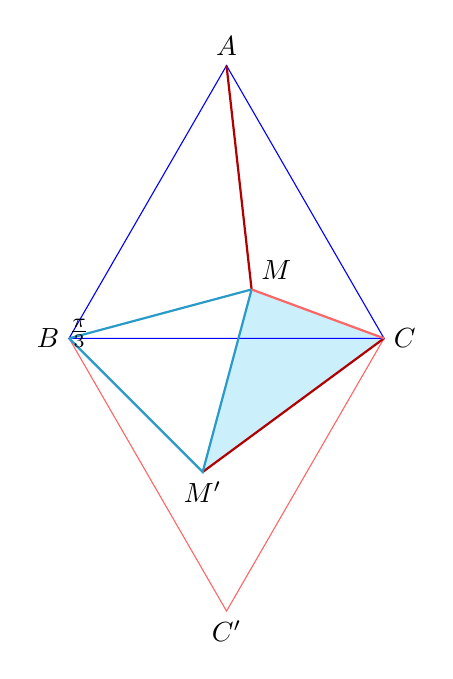
\begin{tikzpicture}[scale = 4]
      \draw (0,0) coordinate(B) node[left] {$B$}
        (1,0) coordinate(C) node[right]{$C$}
        (60:1) coordinate(A) node[above] {$A$}
        (-60:1) coordinate(C') node[below] {$C'$}
        (15:0.6) coordinate(M)node[above right]{$M$}
        (-45:0.6) coordinate(M')node[below]{$M'$};
      \fill [cyan,opacity=0.2] (C) -- (M) -- (M');
      \draw [blue] (B) -- (C) -- (A) -- cycle;
      \draw [red!60] (B) -- (C') -- (C);
      \draw [thick,red!70!black] (A) -- (M) (C) -- (M');
      \draw [thick,cyan!80!black] (B) -- (M)(M) -- (M') -- (B);
      \draw [thick,red!60] (C) -- (M);
      \tkzLabelAngle[pos=0.18](M',B,M){$\frac\pi3$}
      \tkzMarkAngle[cyan,size=0.1cm,mark=none](M',B,M)
    \end{tikzpicture}
    \caption{Pompeiu定理}\label{fig5.2}
  \end{minipage}
\end{figure}

\begin{solution}
  设$r=r_{B,-\frac\pi3}$表示绕着点$B$的角度为$\frac\pi3$的顺时针旋转. 则$r(A)=C,r(C)=C',r(M)=M'$,且点$B$是固定的. 我们有$\triangle MBM'$是等腰三角形,且由于$\angle  B=\frac\pi3$,我们得到$\triangle MBM'$是等边的. 因此,$\triangle CMM'$的边长等于线段$[MC],[MB]$和$[MA]$. 注意到$\triangle CMM'$是退化的,当且仅当$M$在$\triangle ABC$的外接圆上(图 \ref{fig5.2}).
\end{solution}

\begin{solution}
  设$r=r_{A,\frac\pi3}$表示绕着点$A$的角度为$\frac\pi3$的逆时针旋转,且令$C'=r(C),M'=r(M)$,其中$M$是$\triangle ABC$所在平面的任一点. 我们有$MA+MB+MC=BM+MM'+M'C'\ge BC'$,等号成立当且仅当点$B,M,M'$和$C'$是共线的. 由于$\triangle AMM'$是等边三角形,我们得到$\angle AMB=120^\circ,\angle AM'C'=120^\circ$.
  于是$\angle AMB=\angle AMC=120^\circ$. Torricelli点$T$的构造如下:我们在$\triangle ABC$外构造等边三角形$\triangle ACC'$和$\triangle AB'B$,我们有$\{T\}=BC'\cap CB'$(图 \ref{fig5.3}).
\end{solution}

\begin{figure}[!ht]
  \centering
  \caption{Torricelli点}\label{fig5.3}
  \begin{tikzpicture}[scale = 4]
    \tkzDefPoints{0/0/B, 1.1/0/C, 0.22/1/A, 0.6/0.26/M}
    \tkzDefEquilateral(B,A)
    \tkzGetPoint{B'}
    \tkzDefEquilateral(A,C)
    \tkzGetPoint{C'}
    \tkzDefEquilateral(A,M)
    \tkzGetPoint{M'}
    \tkzInterLL(C,B')(B,C')
    \tkzGetPoint{T}
    \draw [thick, red!60!black] (A) -- (T) (B) -- (T) (C) -- (T);
    \draw [thick, blue!70!black] (A) -- (B) -- (C) -- (A);
    \draw [blue] (A) -- (B') -- (B) (A) -- (C') -- (C) (A) -- (M) (B) -- (M) (C) -- (M) (A) -- (M') (M) -- (M') (C') -- (M');
    \draw [red!70!black] (B') -- (T) (C') -- (T);
    \tkzLabelPoints[below](B,C,T)
    \tkzLabelPoints[above](A)
    \tkzLabelPoints[above left=-5pt](B')
    \tkzLabelPoints[above right=-5pt](C')
    \tkzLabelPoints[below left](M')
    \tkzLabelPoints[right](M)
  \end{tikzpicture}
\end{figure}

